% This is a LaTeX thesis template for Monash University.
% to be used with Rmarkdown
% This template was produced by Rob Hyndman
% Version: 6 September 2016

\documentclass{monashthesis}

%%%%%%%%%%%%%%%%%%%%%%%%%%%%%%%%%%%%%%%%%%%%%%%%%%%%%%%%%%%%%%%
% Add any LaTeX packages and other preamble here if required
%%%%%%%%%%%%%%%%%%%%%%%%%%%%%%%%%%%%%%%%%%%%%%%%%%%%%%%%%%%%%%%

\author{Nicholas S Spyrison}
\title{Dynamic visualization of high-dimensional data via low-dimension projections and sectioning across 2D and 3D display devices}
\degrees{B.Sc. Statistics, Iowa State University}
\def\degreetitle{Doctor of Philosophy}
% Add subject and keywords below
\hypersetup{
     %pdfsubject={The Subject},
     %pdfkeywords={Some Keywords},
     pdfauthor={Nicholas S Spyrison},
     pdftitle={Dynamic visualization of high-dimensional data via low-dimension projections and sectioning across 2D and 3D display devices},
     pdfproducer={Bookdown with LaTeX}
}


\bibliography{thesisrefs}

\begin{document}

\pagenumbering{roman}

\titlepage

{\setstretch{1.2}\sf\tighttoc\doublespacing}

\hypertarget{spinifex-manual-control-of-dynamic-linear-projections-of-high-dimensional-data}{%
\chapter{spinifex: manual control of dynamic linear projections of high-dimensional data}\label{spinifex-manual-control-of-dynamic-linear-projections-of-high-dimensional-data}}

\hypertarget{abstract}{%
\section{Abstract}\label{abstract}}

The class of dynamic linear projections that are collectively known as `tours' provide a unique dynamic visualization of numeric multivariate data. Tours are particularly useful for understanding the structure held within multivariate data, and in association with techniques for dimension reduction, supervised, and unsupervised classification. The \emph{R} package \emph{tourr} offers a variety of path generators and geometric displays for conducting tours. This paper discusses an extension package, \emph{spinifex}, that adds support for the path generation of manual tours and extends the display of tours to use with the contemporary animation packages, \emph{plotly} and \emph{gganimate}. Manual tours are used to explore the sensitivity of structure as the contributions of a manipulation variable are changed. This particularly useful after identifying a feature of interest.

A recent paper \{\textcite{wang_mapping_2018}\} visualizes the sensitivey of the hadronic experiments to nucleon structure. Sensitivity was characterized in non-linear 3D embeddings of the first 10 principal components. This research applies manual tours to this data showing that manual tours resolves more structrual information that is orthogonal to the original viewing plane.

Keywords: manual tour, guided tour, grand tour, projection pursuit, high dimensional data, multivariate data, data visualization, statistical graphics, data science.

\hypertarget{introduction}{%
\section{Introduction}\label{introduction}}

A tour is a multivariate data analysis technique in which a sequence of linear (orthogonal) projections are viewed as an animation while the orientation of the projection basis is rotated across time. Each frame of the sequence corresponds to a small change in the projection for a smooth transition that perseveres continuity.

While there are numerous methods that generate tour paths, this research focuses on the manual tour. The manual tour was described in \textcite{cook_manual_1997} and allows a user to control the projection coefficients of a select variable has in a 2D projection. The manipulation of these coefficients allows the analyst to explore how sensitive the projections structure is to these changes. This makes manual tours particularly useful once a feature of interest has been identified, for example, with the use of a guided tour \autocite{cook_grand_1995}. The path of a guided tour is selected via projection pursuit, the optimization of an index function on the projection via a hill climbing algorithm. This allows guided tours to identify interesting projection features rapidly given the relatively large parameter-space. Once the given projection has been provided, it is time to define the path of rotation.

Ideally, the path would be intuitively user-generated from physical movement, be it through mouse or motion capture. Unfortunately, this type of dynamic control has proven difficult to capture for in R. Because of this, manual tours were not implemented in \emph{tourr}. This research allows for the consumption, but not the generation, of such dynamic input. After the capture of an oblique user motion, the rotation needs to be applied to step 3 (rotation sequence) of the algorithm discussed below. In the section below we stick with a radial rotation where, \(\theta\), the angle of in-projection-plane rotation is held constant.

Spinifex utilizes two new animation packages, \emph{plotly} \autocite{sievert_plotly_2018} and \emph{gganimate} \autocite{pedersen_gganimate:_2019}, to display tours, manual or other saved tours. From a given projection, the user can choose which variable to control, and the animation sequence is generated to remove the variable from the projection, and then extend its contribution to be the sole variable in one direction. This allows the viewer to assess the change in structure induced in the projection by the variable's contribution.

The paper is organized as follows. Section \ref{sec:algorithm} explains the algorithm using a toy dataset. Section \ref{sec:display} discussed the display of the animation after the path has been generated. Section \ref{sec:application} illustrates how this can be used for sensitivity analysis applied to contemporary high energy physics. The last section, \ref{sec:discussion} summarizes the work and discusses future research.

\hypertarget{sec:algorithm}{%
\section{Algorithm}\label{sec:algorithm}}

The section below describes the algorithm for performing a 2D radial manual tour:

\begin{enumerate}
\def\labelenumi{\arabic{enumi}.}
\tightlist
\item
  Provided with a 2D projection, choose a variable to explore. This is called the ``manip'' variable.
\item
  Create a 3D manipulation space, where the manip variable has the full contribution.
\item
  Generate a rotation sequence which increases the norm of the coefficient to 1 and zeros it.
\end{enumerate}

The steps are described in more detail below. The R functions used below mentioned briefly, but more complete code example can be found in section \ref{sec:usage}

\hypertarget{notation}{%
\subsection{Notation}\label{notation}}

This section describes the notation used in the algorithm for a 2D radial manual tour.

\begin{itemize}
  \item $\textbf{X}$, the data, an $n \times p$ numeric matrix to be embedded in two dimensions.
  \item $\textbf{B} = (B_1,~ B_2)$, any of orthonormal projection basis set, $p \times 2$ matrix, describing the projection from $p$ to two dimensions
  \item $\textbf{e}$, a zero column vector of length $p$ with the $k-$th element set to one, where $k$ is the number of the variable to manipulate.
  \item $\theta$, the angle of in-projection-plane rotation, for example, on the reference axes. 
  \item $\phi$, the angle of out-of-projection-plane rotation, coming into the manipulation space.
\end{itemize}

The algorithm primarily operates on the projection basis and utilizes the data only when making a display. The projection space can be viewed at any point in the process by pre-multiplying the data and plotting the first 2 variables.

\hypertarget{toy-data-set}{%
\subsection{Toy data set}\label{toy-data-set}}

The flea data, originally from \textcite{lubischew_use_1962}, available in the R package \emph{tourr} \autocite{wickham_tourr_2011} is used to illustrate the algorithm. The data contains 74 observations across 6 variables, physical measurements of the flea beetles. Each observation belonging to one of three species.

The data is defined. A basis set (ideally that views an interesting feature) should be provided to explore the sensitivity of the variables to the structure. To identify a projection containing an interesting feature, apply
a guided tour\autocite{cook_interactive_2007} on the flea data. In a guided tour the projection sequence is selected by optimizing an index via hill-climbing. In this case, the holes index is selected. The holes index is maximized by when the projected observations are furthest from the center. Figure \ref{fig:step0} shows a locally optimized projection for this data. The left plot displays the reference axes of the projection basis, a visual indication of the magnitude and direction each variable contributed to the projections. The right plot shows the projection of the data through the basis set described by the reference axes (left). Data points are colored and given point characters according to the species of the flea (the guided tour was unsupervised with this information).



\begin{figure}

{\centering 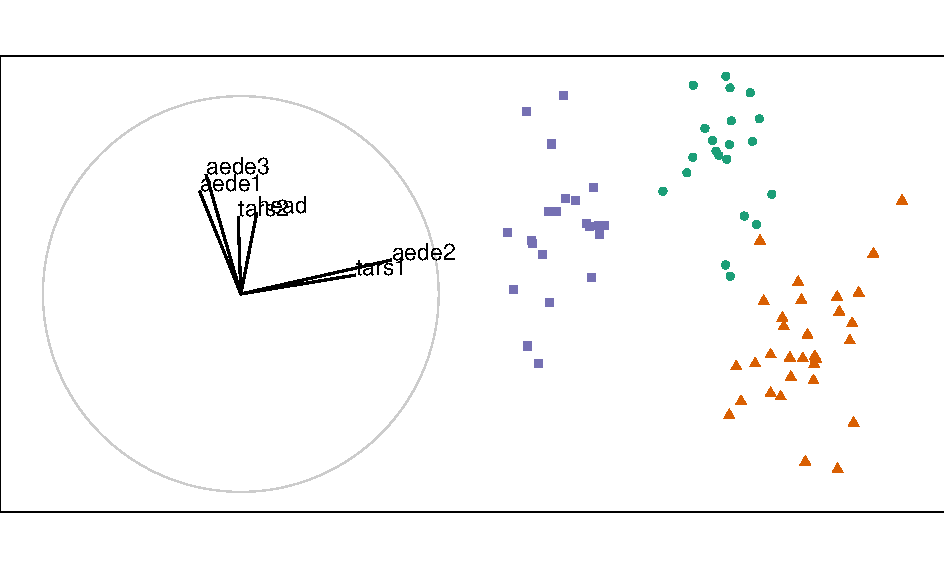
\includegraphics[width=0.95\linewidth]{confirmation_report_ns_files/figure-latex/step0-1} 

}

\caption{Basis reference axes (left) and projected data (right) of standardized flea data. Data points color and shape are mapped to beetle species. Basis identified by a holes-index guided tour. The variables \texttt{aede2} and \texttt{tars1} contribute mostly orthogonal to the other variables. We'll select \texttt{aede2} as our manipulation variable to see how the structure of the projection changes as we rotate \texttt{aede2} into and out of the projection.}\label{fig:step0}
\end{figure}

Call \texttt{view\_basis()} on a basis to produce a \emph{ggplot2} graphic similar to \ref{fig:step0}. Projection space is always available for display via the matrix multiplication \(\textbf{X}_{[n,~p]} ~*~ \textbf{B}_{[p,~d]} ~=~ \textbf{P}_{[n,~d]}\).

\hypertarget{step-1-choose-variable-of-interest}{%
\subsection{Step 1) Choose variable of interest}\label{step-1-choose-variable-of-interest}}

In figure \ref{fig:step0}, above, the contributions of the variables \texttt{tars1} and \texttt{aede2} are mostly orthogonal to the contributions of the other four variables. These two variables explain the variation of the data between the purple and green species. We select \texttt{aede2} as the manip var, the variable to be manipulated as it typically has a larger contribution after the optimizing the holes index. The question that will be explored in the explanation of the algorithm is how important the variable \texttt{aede2} is to the separation of the clusters.

\hypertarget{step-2-create-the-manip-space}{%
\subsection{Step 2) Create the manip space}\label{step-2-create-the-manip-space}}

Initialize a zero vector \(e\) of \(p\) elements. Because \texttt{aede2} is the fifth variable in the data, set the \(k=5\)-th element to one giving the manip var a full contribution in this dimension. Use the Gram-Schmidt process to orthonormalize the zero vector onto the basis yielding the 3D manipulation space, \textbf{M}.

\begin{align*}
  \textbf{e} &\leftarrow Orthonormalize_{GS}(\textbf{e}) w.r.t. Basis \\
  &= \textbf{e} - \langle \textbf{e},\textbf{B}_1 \rangle \textbf{B}_1 - \langle \textbf{e}, \textbf{B}_2 \rangle \textbf{B}_2 \\
  \\
  \textbf{M}_{[p,~3]} &= (\textbf{B}_1,\textbf{B}_2,\textbf{e})
\end{align*}

Adding this extra dimension to our basis plane allows for the coefficients of the specified variable to be changed. For example, the ability to lift a piece of paper, rather than being constrained to the motion on a table top. Orthonormalizing rescales the new depth vector while the projection down to 2D is the original basis, that is the first \(d\) vectors remain constant. Imagine the reference axes (and projection plane) laying flat on a table, while a new dimension exists with axes projecting back onto the reference axes. An illustration of such can be seen below in figure \ref{fig:step2}. The manip var is highlighted, while the depths of the other variables are not depicted.



\begin{figure}

{\centering 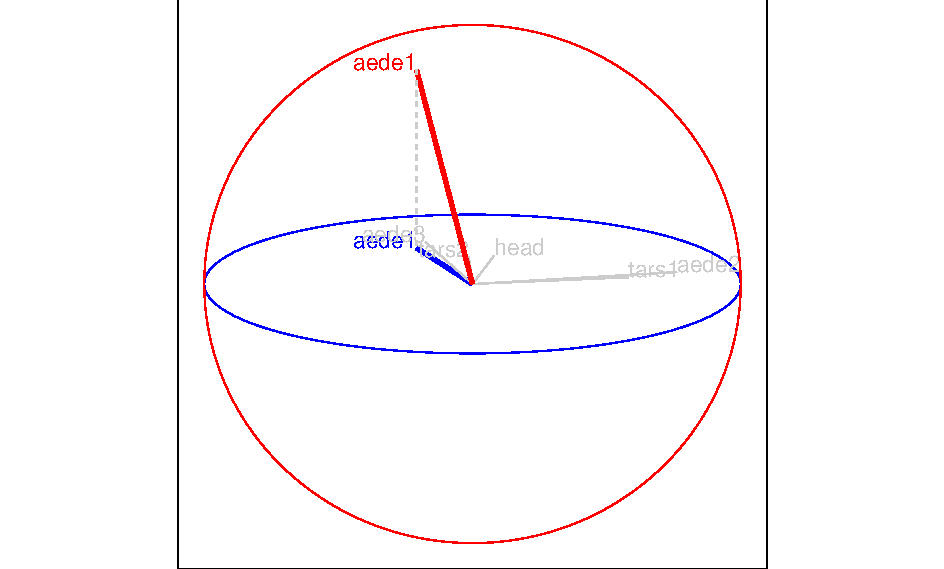
\includegraphics[width=1\linewidth]{confirmation_report_ns_files/figure-latex/step2-1} 

}

\caption{Manipulation space for controlling the contribution of \texttt{aede2} of standardized flea data. Basis selected by a holes-index guided tour. The Projection plane is shown in blue. The manipulation axis, in red, allows the coefficients of the manip var to be changed.}\label{fig:step2}
\end{figure}

The representation in \ref{fig:step2} can be duplicated by calling the function \texttt{view\_manip\_space()}.

\hypertarget{step-3-generate-rotation}{%
\subsection{Step 3) Generate rotation}\label{step-3-generate-rotation}}

Imagine holding the red axis it is fixed to the origin. As it is manipulated the projection back onto the projection plane correspondingly moves. This is what happens in a manual tour. For a radial tour, fix \(\theta\), the angle within the blue plane, and vary the sequence of \(\phi\), the angle coming out of the projection plane. Conceptually, live manipulation on a 2D plane allows the user to dynamically control these angles, effectively changing the coefficients of the manip var, which then performs a constrained rotation on the remaining variables.

For the demonstration of the radial tour, we define a sequence for \(\phi\) that brings the initial contribution of the manip var to be maximized and then zeroed before returning to the initial position.

\textbf{For } \(i\) \textbf{in 1 to n\_slides:}

Post-multiply the manipulation space by the pre-defined rotation matrix producing \textbf{RM}, the rotated manip space.

Let:

\begin{description}
  \item[$c_\theta$] be the cosine of $\theta$
  \item[$c_\phi$]   be the cosine of $\phi$
  \item[$s_\theta$] be the sine of   $\theta$
  \item[$s_\phi$]   be the sine of   $\phi$
\end{description}

then
\begin{align*}
  \textbf{RM}_{[p,~3,~i]}
  &= \textbf{M}_{[p,~3]} ~*~ \textbf{R}_{[3,~3]} \\
  &= \begin{array}{cc}
    M_{1,~1} & M_{1,~2} & M_{1,~3} \\
    M_{2,~1} & M_{2,~2} & M_{2,~3} \\
    \vdots   & \vdots   \\
    M_{p,~1} & M_{p,~2} & M_{p,~3}
  \end{array}_{[p,~3]}
    ~*~
  \begin{array}{ccc}
    c_\theta^2 c_\phi s_\theta^2 &
    -c_\theta s_\theta (1 - c_\phi) &
    -c_\theta s_\phi \\
    -c_\theta s_\theta (1 - c_\phi) &
    s_\theta^2 c_\phi + c_\theta^2 &
    -s_\theta s_\phi \\
    c_\theta s_\phi &
    s_\theta s_\phi &
    c_\phi
  \end{array}_{[3,~3]}
\end{align*}

A note on application: compile the sequence of \(\phi_i\) and create an array/long table for each rotated manipulation space. \(\phi\) is the angle relative to the initial value of \(\phi\), we find the transformation \(\phi_i\) - \(\phi_1\) useful to think about \(\phi\) relative to the basis plane. Additionally, the value of \(\phi\) may be offset by a factor of pi. If the manip variable doesn't move as expected these are the first places to check.

\begin{Shaded}
\begin{Highlighting}[]
\ControlFlowTok{for}\NormalTok{ (phi }\ControlFlowTok{in} \KeywordTok{seq}\NormalTok{(seq_start, seq_end, phi_inc_sign)) \{}
\NormalTok{  slide <-}\StringTok{ }\NormalTok{slide }\OperatorTok{+}\StringTok{ }\DecValTok{1}
\NormalTok{  tour[,, slide] <-}\StringTok{ }\KeywordTok{rotate_manip_space}\NormalTok{(manip_space, theta, phi)[, }\DecValTok{1}\OperatorTok{:}\DecValTok{2}\NormalTok{]}
\NormalTok{\}}
\end{Highlighting}
\end{Shaded}

Figure \ref{fig:step3} illustrates a sequence with 15 projected bases and highlight the manip variable on top while showing the corresponding projected data points on the bottom. Take note of how the changes in the manip var change the distance between the purple and green cluster of points, \texttt{aede2} is crucial in distinguishing between these groups. Tours are typically viewed as an animation such a dynamic version of this tour can be viewed online at \url{https://nspyrison.netlify.com/thesis/flea_manualtour_mvar5/}. The page may take a moment to load. The format of this figure and linking to an HTML animation will be used again in the Application, section \ref{sec:application}.



\begin{figure}

{\centering 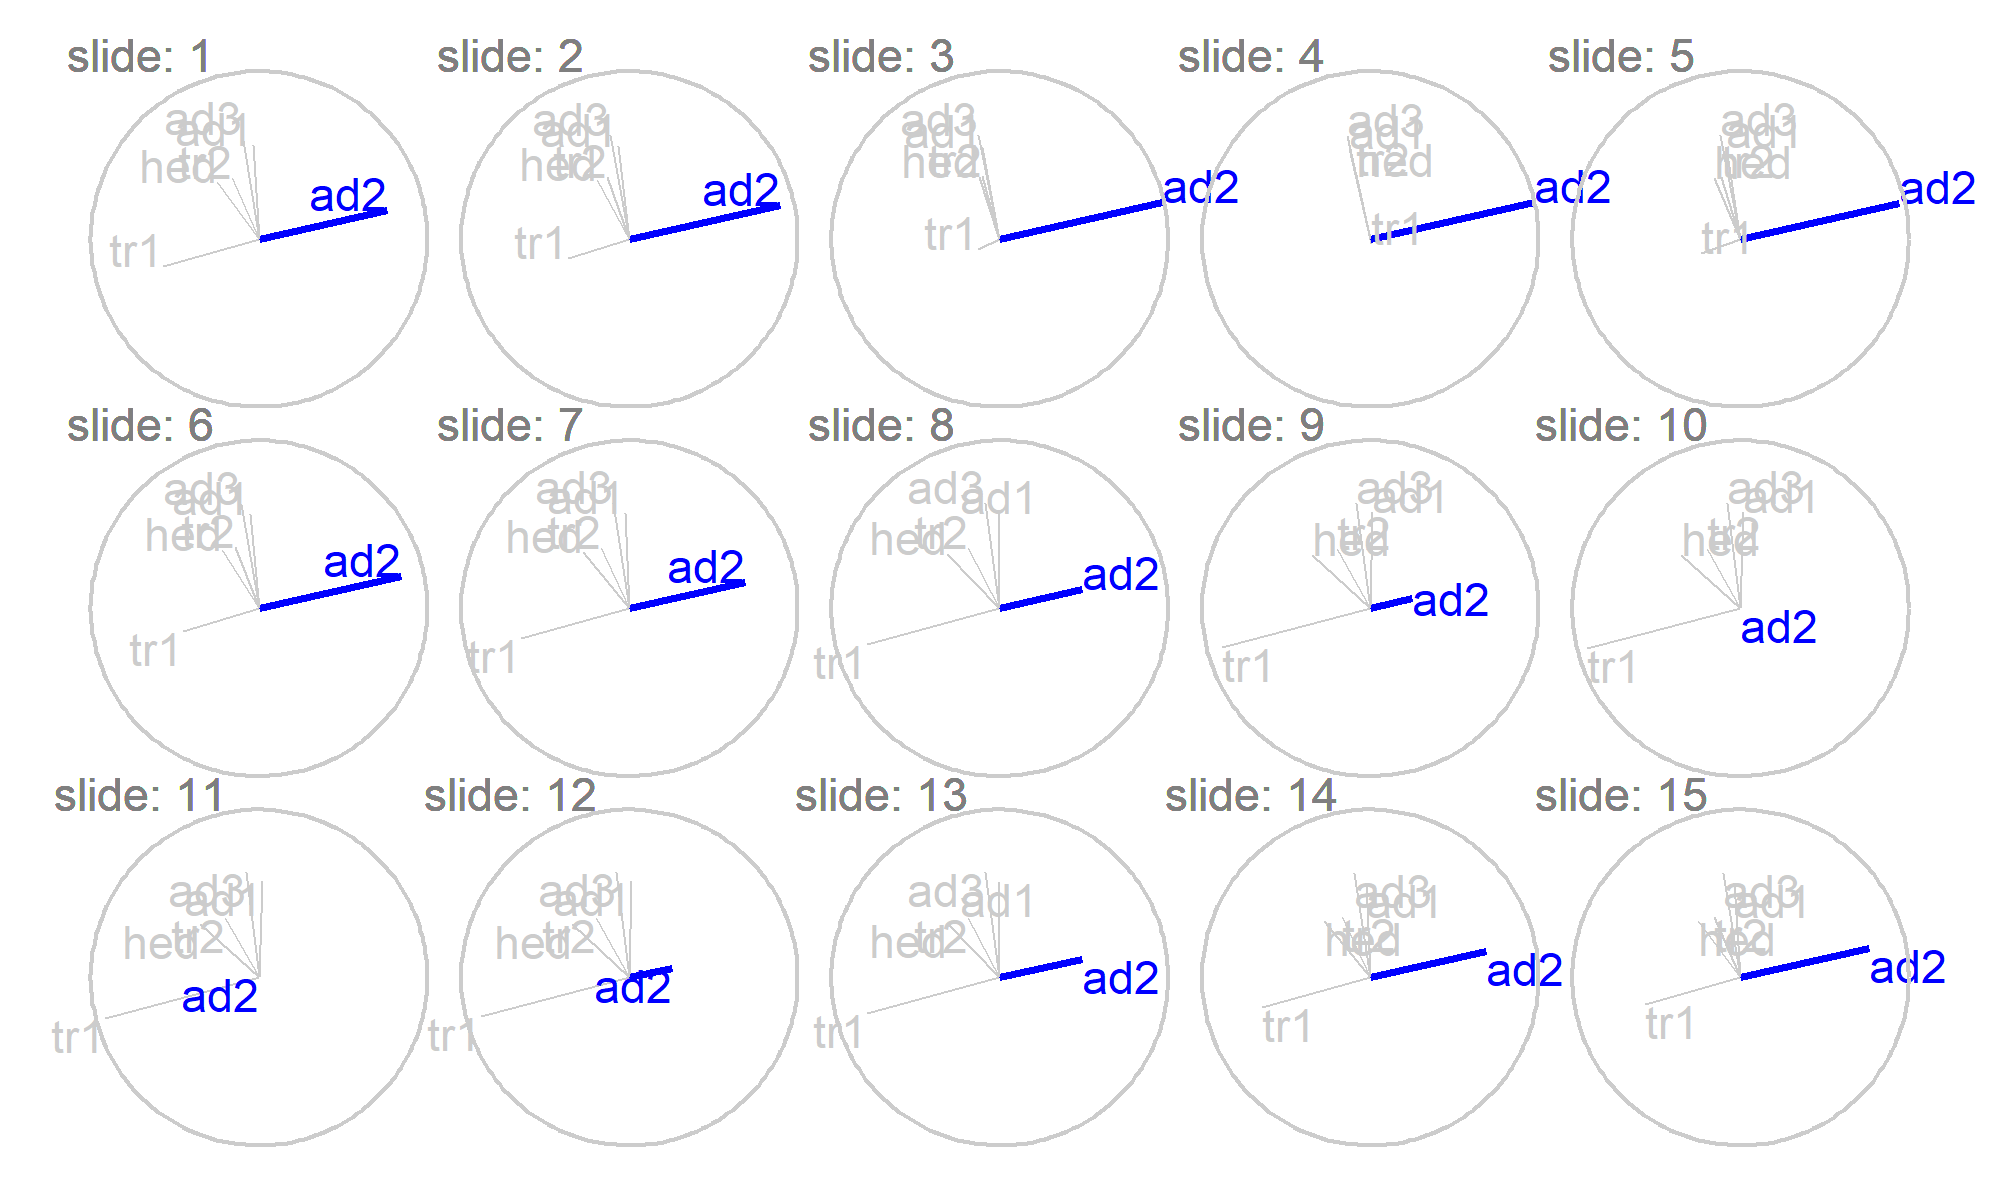
\includegraphics[width=6in,height=7.2in]{./output/step3_manual_tour.} 

}

\caption{Radial manual tour changing the contributions from \texttt{aede2} of standardized flea data. The contributions increase from its initial contribution to a full contribution to the projection before decreasing to zero and then returning to its initial value. The change in the projected data shows that \texttt{aede2} is important for distinguishing between the purple and green clusters. An animated version can be viewed at \url{https://nspyrison.netlify.com/thesis/flea_manualtour_mvar5/}.}\label{fig:step3}
\end{figure}

Animations can be produced using the function \texttt{play\_manual\_tour()}. This function defaults to an HTML5 widget produced from \emph{plotly}.

\hypertarget{sec:display}{%
\section{Data in projection-space}\label{sec:display}}

In light of performance, the above operations are performed on the bases without the use of the larger datasets. After the bases are brought into the projection-space, however, it is helpful to observe them with data in the same space. Pre-multiply the data by basis frame bringing the data into the projection space.

\begin{align}
  \textbf{P}_{[n,~3]}
    &= \textbf{X}_{[n,~p]} ~*~ \textbf{RM}_{[p,~3]} \\
    &=
      \begin{bmatrix}
          X_{1,~1} & \dots & X_{1,~p} \\
          X_{2,~1} & \dots & X_{2,~p} \\
          \vdots   & \vdots & \vdots  \\
          X_{n,~1} & \dots & X_{n,~p}
      \end{bmatrix}_{[n,~p]}
      ~*~
      \begin{bmatrix}
        RM_{1,~1} & RM_{1,~2} & RM_{1,~3} \\
        RM_{2,~1} & RM_{2,~2} & RM_{2,~3} \\
        \vdots     & \vdots     & \vdots  \\
        RM_{p,~1} & RM_{p,~2} & RM_{p,~3}
      \end{bmatrix}_{[p,~3]}
\end{align}

For a 2D scatterplot, plot the first two variables from each frame statically as in the previous figure, or in sequence, producing an animated scatterplot. The remaining variable is sometimes linked to a data point aesthetic (such as size or color) to produce depth cues used in conjunction with the \(XY\) scatterplot.

\hypertarget{rendering-and-sharing}{%
\subsection{Rendering and sharing}\label{rendering-and-sharing}}

The \emph{tourr} package utilizes R's base graphics for the display of tours. \emph{spinifex} allows tours to be used in rendered in \emph{plotly} \textcite{sievert_plotly_2018} as an HTML5 object or \emph{gganimate} \textcite{pedersen_gganimate:_2019} as .gif or .mp4 objects. Both of which build off \emph{ggplot2} objects in internal functions. Sharing of animations is not trivial especially in print and static formats such as .pdf. Even with the use of computers and dynamic file formats capturing the correct resolution, aspect, and display is challenging and many formats quickly bloat file sizes. Keep in mind hosting options and exporting functions from \emph{plotly}, \emph{gganimate} and \emph{tourr}.

\hypertarget{storage}{%
\subsection{Storage}\label{storage}}

Storing each data point for every frame of the animation is very inefficient. Just as operations are performed on the bases, so too should tour paths be stored as bases. Consider a radial manual tour, we can store the salient features in 3 bases, where \(\phi\) is at its starting, minimum, and maximum values. The frames in between can be interpolated by supplying angular speed. With the use of the \texttt{tourr::save\_history()} function, the target bases can be saved. From there geodesic interpolation can be used to populate the intermittent frames. This type of interpolation should not be used on manual tours, which have already been initialized into a 3D manipulation space where direct linear interpolation is appropriate.

\hypertarget{sec:application}{%
\section{Application}\label{sec:application}}

In a recent paper, \textcite{wang_mapping_2018}, the authors aggregate and visualize the sensitivity of hadronic experiments to ncleon structure. The authors introduce a new tool, PDFSense, to aid in the visualization of Parton distribution functions (PDF). The parameter-space of these experiments lies in 56 dimensions, \(\delta \in \mathbb{R}^{56}\), and are visualized as 3D subspaces of the 10 first principal components in linear (PCA) and non-linear (t-SNE) embeddings.

Using the same data, another study, \textcite{cook_dynamical_2018}, applies grand tours to the same subspaces. Grand tours are able to better resolve the distribution shape of clusters, intra-cluter detail, better outlier detection, and exonerate a claim persened from TFEP (TensorFlow embedded projections). Table 1 of Cook et al.~summarizes the key findings of observations made with PDFSense \& TFEP and those from grand tours.

Without getting too domain-specific the data has three primary groupings; DIS, VBP, and jet Each group is a particular class of experiments and each with many experimental datasets which inturn have many observation. Inconsideration of data density and business of the data We conduct manual tours on a subsets of the DIS and jet clusters. This explores the sensitivity of the structue to each of the variables in turn, and we present the subjectively best and worst manaul tour identifying structure in the respective data sets.

\hypertarget{jet-cluster}{%
\subsection{Jet cluster}\label{jet-cluster}}

The jet cluster is of interest as it contains the largest data sets and is found to be important in \textcite{wang_mapping_2018} The jet cluster resides in a smaller dimensionality than the full set of experiments with 4 principal components explaining 95\% of the variation in the jet cluster \autocite{cook_dynamical_2018}. The data is subset down to ATLAS7old and ATLAS7new to focus in on two groups with a reasonable number of observations that occupy different parts of the subspace. Below, we perform radial manual tours all four principal components within this scope. Visualizing PC3 and PC4 in figure \ref{fig:JetClusterGood} (more sturcturally insightful) and figure \ref{fig:JetClusterBad} (less sturcturally insightful) respectively, and list links to dynamic animation of all variables.



\begin{figure}

{\centering 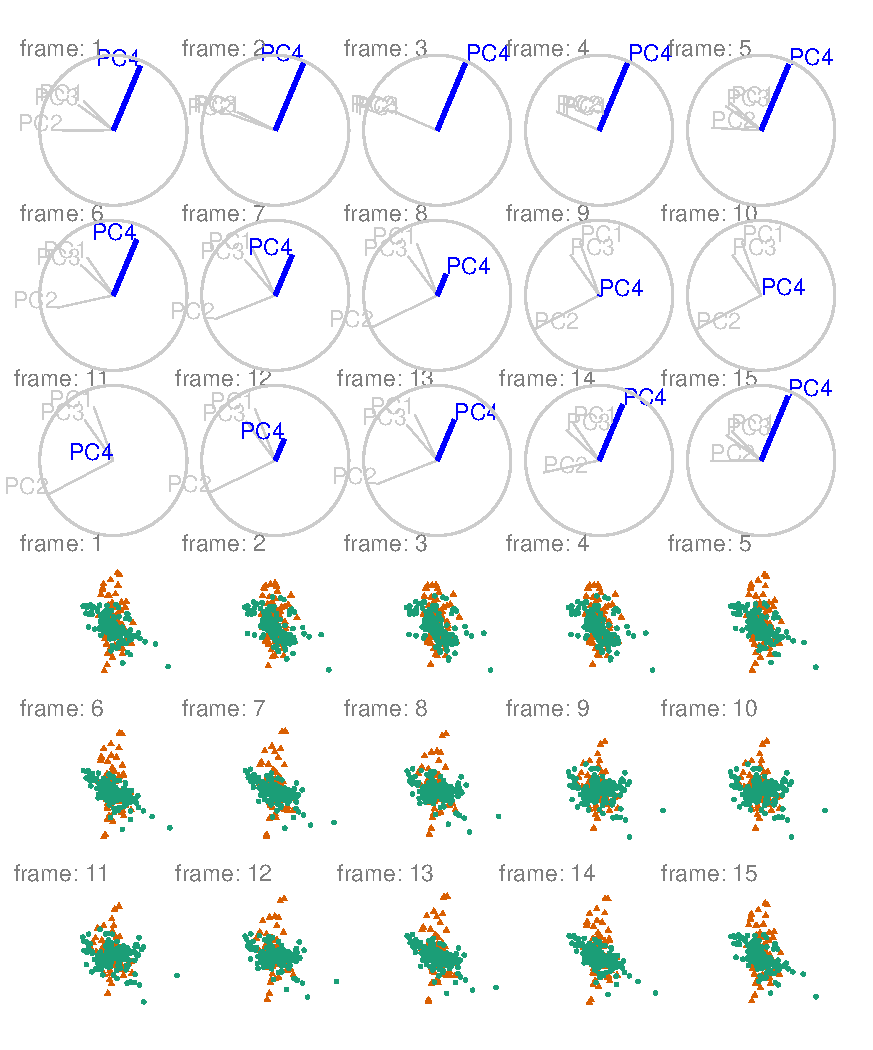
\includegraphics[width=6in,height=7.2in]{./figures/JetClusterGood} 

}

\caption{Jet cluster, a radial manual tour of PC3. Colored by experiment type: `ATLAS7new' in green and `ATLAS7old' in orange. When PC3 fully contributes to the projection ATLAS7new (green) occupies unique space and several outliers are identifiable. Zeroing the contribution from PC3 to the projection hides the outliers and indeed all observations with ATLAS7new are contained within ATLAS7old (orange). A dynamic version can be viewed at \url{https://nspyrison.netlify.com/thesis/jetcluster_manualtour_pc3/}.}\label{fig:JetClusterGood}
\end{figure}



\begin{figure}

{\centering 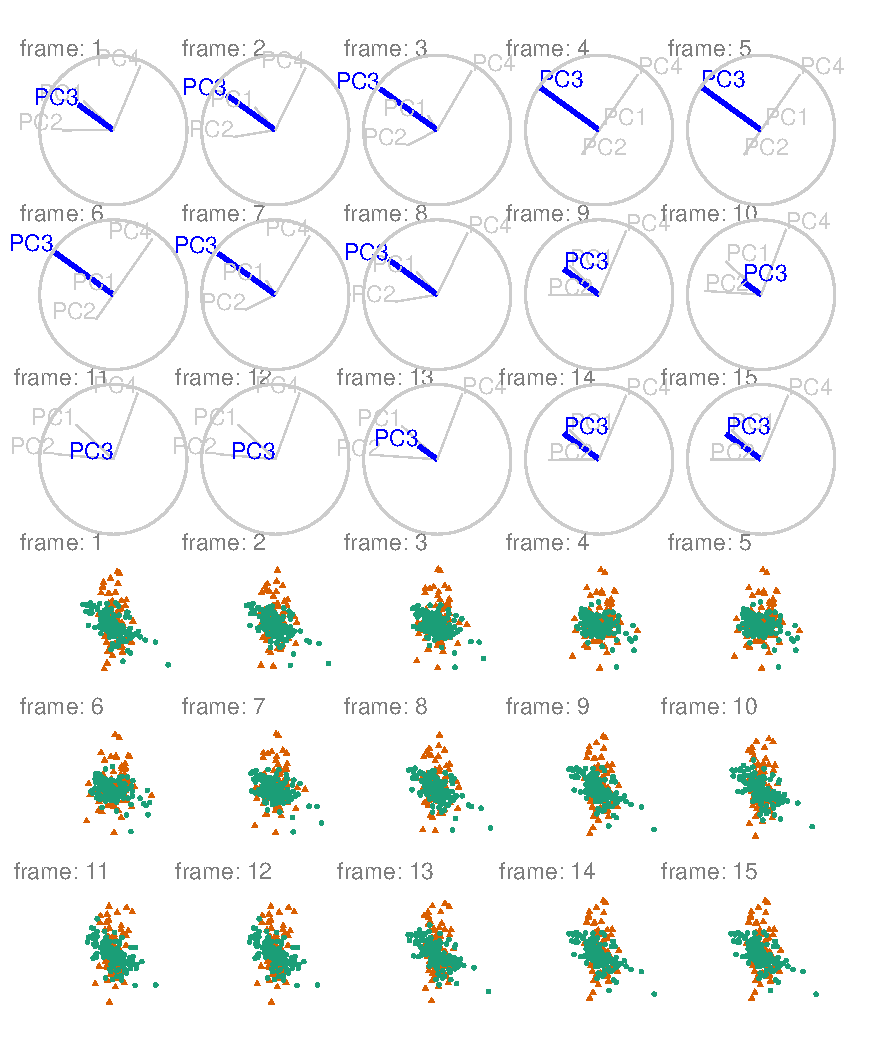
\includegraphics[width=6in,height=7.2in]{./figures/JetClusterBad} 

}

\caption{Jet cluster, a radial manual tour of PC4. Colored by experiment type: ATLAS7new in green and ATLAS7old in orange. This manual tour contains less interesting information ATLAS7new (green) has points that are right and left of ATLAS7old, while most points occupy the same projection space, regardless of the contribution of PC4. A dynamic version can be viewed at \url{https://nspyrison.netlify.com/thesis/jetcluster_manualtour_pc3/}.}\label{fig:JetClusterBad}
\end{figure}

\hypertarget{todo-edit-application-grammarly-and-word-checks.}{%
\section{TODO: edit application, Grammarly and word checks.}\label{todo-edit-application-grammarly-and-word-checks.}}

Manipulating PC3, where varying the angle of rotation brings interesting features into and out of the center mass of the data, is more interesting than the manipulation of PC4, where the features are mostly independent of the contribution of PC4.

Jet cluster manual tours manipulating each of the principal components can be viewed from the links: \href{https://nspyrison.netlify.com/thesis/jetcluster_manualtour_pc1/}{PC1}, \href{https://nspyrison.netlify.com/thesis/jetcluster_manualtour_pc2/}{PC2}, \href{https://nspyrison.netlify.com/thesis/jetcluster_manualtour_pc3/}{PC3}, and \href{https://nspyrison.netlify.com/thesis/jetcluster_manualtour_pc4/}{PC4}.

\hypertarget{dis-cluster}{%
\subsection{DIS cluster}\label{dis-cluster}}

We perform a manual tour on this data, manipulating PC6 as depicted in figure \ref{fig:DISclusterGood}. Looking at several frames we see that DIS HERA data lies mostly on a plane. When PC6 has full contributions, we see the dimuon SIDIS in purple is almost orthogonal to the DIS HERA (green). Yet the contribution of PC6 has zeroed the dimuon SIDIS data occupy the same space as the DIS HERA data. A dynamic version of this manual tour can be found at:
\url{https://nspyrison.netlify.com/thesis/discluster_manualtour_pc6/}.
The page may some time to load, as the animation is several megabytes.



\begin{figure}

{\centering 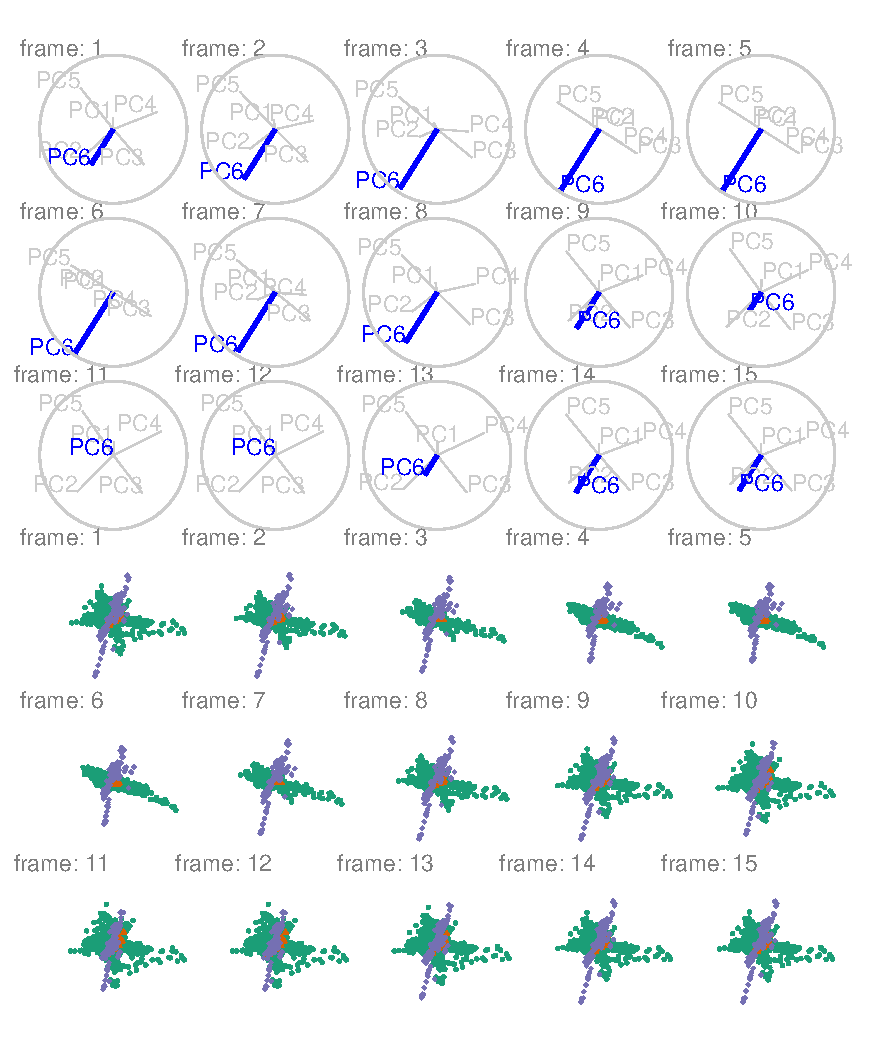
\includegraphics[width=6in,height=7.2in]{./figures/DISclusterGood} 

}

\caption{DIS cluster, a radial manual tour of PC6. colored by experiment type: `DIS HERA1+2' in green, `dimuon SIDIS' in purple, and `charm SIDIS' in orange. When the contribution PC 6 is large we see that dimuon SIDIS (purple) data are nearly orthogonal to DIS HERA (green) data. As the projection is rotated, we can also see that DIS HERA (green) practically lies on a plane in this 6D subspace. When the contribution of PC6 is near zero, dimonSIDIS (purple) occupies the same space as the DIS HERA data. A dynamic version can be viewed at \url{https://nspyrison.netlify.com/thesis/discluster_manualtour_pc6/}.}\label{fig:DISclusterGood}
\end{figure}

The selection of the correct manip variable is important as the manipulation spaces convey different information. For example, in figure \ref{fig:DISclusterBad} we select PC2 as the manip variable finding it to be less insightful than PC6.



\begin{figure}

{\centering 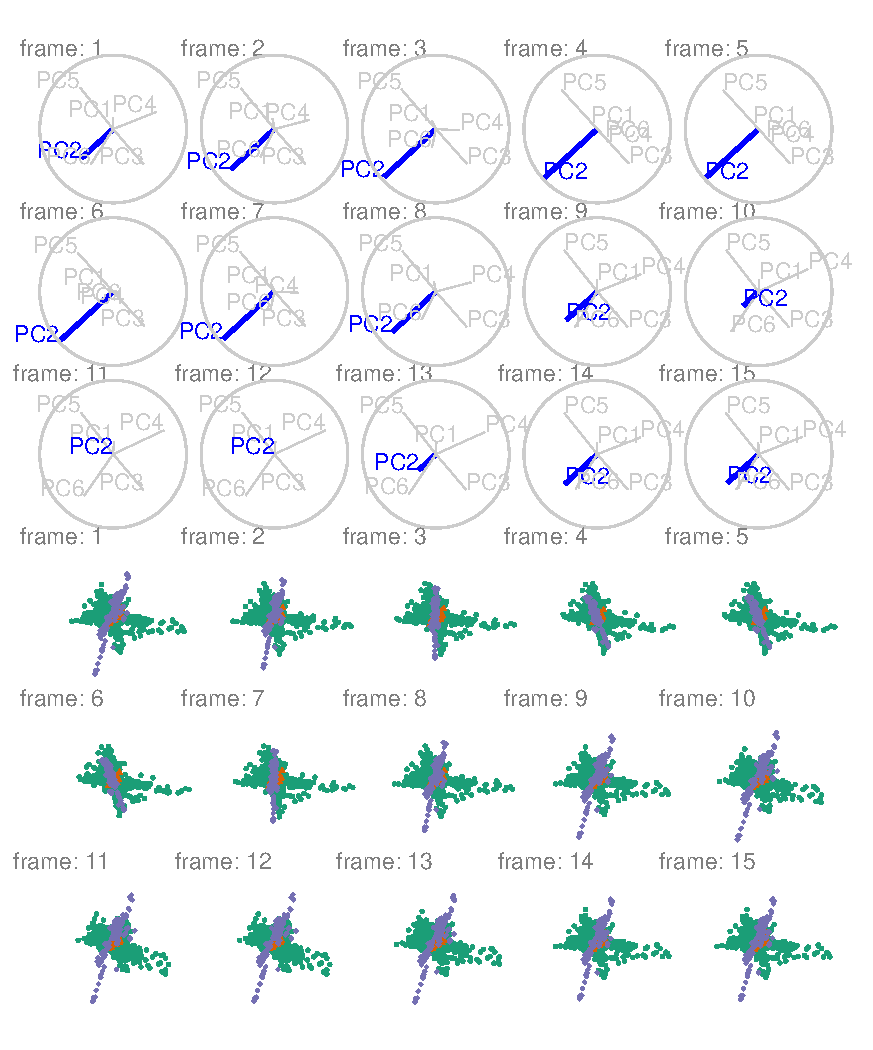
\includegraphics[width=6in,height=7.2in]{./figures/DISclusterBad} 

}

\caption{DIS cluster, a radial manual tour of PC2. Colored by experiment type: `DIS HERA1+2' in green, `dimuon SIDIS' in purple, and `charm SIDIS' in orange. The structure of previously described plane of DIS HERA (green) and nearly orthogonal dimuon SIDIS (purple) is present, however, the manipulating PC2 does not give a head-on view of either, a less useful manual tour than that of PC6. A dynamic version can be viewed at \url{https://nspyrison.netlify.com/thesis/discluster_manualtour_pc2/}.}\label{fig:DISclusterBad}
\end{figure}

DIS cluster manual tours manipulating each of the principal components can be viewed from the links: \href{https://nspyrison.netlify.com/thesis/discluster_manualtour_pc1/}{PC1}, \href{https://nspyrison.netlify.com/thesis/discluster_manualtour_pc2/}{PC2}, \href{https://nspyrison.netlify.com/thesis/discluster_manualtour_pc3/}{PC3}, \href{https://nspyrison.netlify.com/thesis/discluster_manualtour_pc4/}{PC4}, \href{https://nspyrison.netlify.com/thesis/discluster_manualtour_pc5/}{PC5}, and \href{https://nspyrison.netlify.com/thesis/discluster_manualtour_pc6/}{PC6}.

\hypertarget{sec:usage}{%
\section{Source code and usage}\label{sec:usage}}

Use the below code as a guide for installation and finding the vignette. The vignette offers a less technical discussion opting to focus on code usage and goes through a couple more use cases. If you prefer to follow along with the example in the algorithm then simplified code is also listed below.

\begin{Shaded}
\begin{Highlighting}[]
\CommentTok{# devtools::install_github("nspyrison/spinifex") # Development version}
\KeywordTok{install.package}\NormalTok{(}\StringTok{"spinifex"}\NormalTok{)}

\CommentTok{# Also see vignette:}
\KeywordTok{vignette}\NormalTok{(}\StringTok{"spinifex"}\NormalTok{) }\CommentTok{# vignette ‘spinifex’ not found}

\CommentTok{## manual tour of std flea from holes-index:}
\KeywordTok{library}\NormalTok{(spinifex)}
\NormalTok{f_dat  <-}\StringTok{ }\NormalTok{tourr}\OperatorTok{::}\KeywordTok{rescale}\NormalTok{(flea[,}\DecValTok{1}\OperatorTok{:}\DecValTok{6}\NormalTok{])}
\NormalTok{f_cat  <-}\StringTok{ }\KeywordTok{factor}\NormalTok{(flea}\OperatorTok{$}\NormalTok{species)}
\NormalTok{f_path <-}\StringTok{ }\KeywordTok{save_history}\NormalTok{(f_dat, }\KeywordTok{guided_tour}\NormalTok{(}\KeywordTok{holes}\NormalTok{()))}
\NormalTok{f_bas  <-}\StringTok{ }\KeywordTok{matrix}\NormalTok{(f_path[,, }\KeywordTok{max}\NormalTok{(}\KeywordTok{dim}\NormalTok{(f_path)[}\DecValTok{3}\NormalTok{])], }\DataTypeTok{ncol=}\DecValTok{2}\NormalTok{)}
\NormalTok{f_mvar <-}\StringTok{ }\DecValTok{5}
\NormalTok{f_lab  <-}\StringTok{ }\KeywordTok{colnames}\NormalTok{(f_dat)}

\CommentTok{# View the basis}
\KeywordTok{view_basis}\NormalTok{(f_bas, }\DataTypeTok{data =}\NormalTok{ f_dat, }\DataTypeTok{lab =}\NormalTok{ f_lab)}
\CommentTok{# View the manip space}
\KeywordTok{view_manip_space}\NormalTok{(}\DataTypeTok{basis =}\NormalTok{ f_bas, }\DataTypeTok{manip_var =}\NormalTok{ f_mvar, }\DataTypeTok{lab =}\NormalTok{ f_lab)}
\CommentTok{# Play animation as HTML5 widget using plotly}
\KeywordTok{play_manual_tour}\NormalTok{(}\DataTypeTok{data =}\NormalTok{ f_dat, }\DataTypeTok{basis =}\NormalTok{ f_bas, }\DataTypeTok{manip_var =}\NormalTok{ f_mvar, }
                 \DataTypeTok{col =}\NormalTok{ f_cat, }\DataTypeTok{angle =}\NormalTok{ f_angle)}
\end{Highlighting}
\end{Shaded}

\hypertarget{acknowledgments}{%
\subsection{Acknowledgments}\label{acknowledgments}}

This article was created in \emph{R} \autocite{r_core_team_r:_2018}, using \emph{bookdown} \autocite{xie_bookdown:_2016} and \emph{rmarkdown} \autocite{xie_r_2018}, with code generating the examples inline. The source files for this article be found at \href{https://github.com/nspyrison/confirmation/}{github.com/nspyrison/confirmation/}.
The source code for the \emph{spinifex} package can be found at \href{https://github.com/nspyrison/spinifex/}{github.com/nspyrison/spinifex/}.

\hypertarget{sec:discussion}{%
\section{Discussion}\label{sec:discussion}}

Tours, the dynamic linear projection of multivariate data, is an important aspect of data visualization extending the display of data-space as data dimensionality increases. This research has modified the algorithm producing manual tours, applied this functionality in \emph{R} and offers extends the graphics offerings that can be used to display tours. The paragraphs below explore how this work might be extended.

Future research on the algorithm would include extending it for use in 3D projections. The addition of another dimension theoretically allows for improved perception. This could explore interactions in immersive virtual reality or mixed reality, which may further allow for a better perception of structure and aid in higher-dimensional function visualization. Functions with many parameters suffer from the same dimensionality problem as data while their possible values lie on a plane of values rather than discrete points. Occulation, or the closer surface blocking further surfaces, will likely be an issue that may be alleviated by the use of wire mesh, changing opacity, or looking at sections of the projections \autocite{furnas_prosection_1994}.

The \emph{tourr} package provides many other geometric displays with the \texttt{tourr::display\_*()} family. These geometric options could be integrated into the \emph{ggplot2} framework for display on \emph{plotly} and \emph{gganimate}. Additionally, the \emph{animation} package \textcite{xie_animation:_2018} could be implemented for another graphics framework. However, \emph{animation} builds from base graphs while \emph{spinifex} utilizes \emph{ggplot2} graphics.

The Givens rotations and Householder reflections as outlined in \textcite{buja_computational_2005} could also be added. Currently, Gram-Schmidt is the only form of frame interpolation used (not used in manual tours). In a Givens rotation, the \(x\) and \(y\) components (for example \(\theta~= 0,~pi/2\)) of the in-plane rotation are calculated separately and would be applied sequentially to produce the radial rotation. Householder reflections define reflection axes to project points on to the axes and generate rotations.

Having a script only interaction with tours causes a significant barrier to entry. To a lesser extent, \emph{plotly} offers some static interactions with the contained object, such as tooltips, brushing, and linking without communicating back to the R console. The development of a dynamic graphical user interface, perhaps with the use of a \emph{shiny} \autocite{chang_shiny:_2018} application, would mitigate the barrier to entry, allow for more rapid analysis, and offer an approachable demo tool. The user could easily switch between variables to control, adjust interpolation step angle, or flag/save specific frame basis sets.

\printbibliography[heading=bibintoc]



\end{document}
